\documentclass[12pt,a4paper]{article}
\usepackage{fontspec}
\setmainfont{Times New Roman}
\setsansfont{Arial}
\setmonofont{Consolas}[Scale=MatchLowercase]
\usepackage[english,russian]{babel}
\usepackage[margin=20mm]{geometry}
\usepackage{amsmath,amssymb,booktabs,graphicx,float}
\usepackage[section]{placeins}
\usepackage[hidelinks,unicode]{hyperref}
\usepackage{url}
\setlength{\parindent}{1.2em}
\setlength{\parskip}{1pt}
\setlength{\emergencystretch}{2em}
\newcommand{\KL}{\operatorname{KL}}
\newcommand{\PPL}{\operatorname{PPL}}
\title{Фиксированный контекстный учитель для AARTM:\\инициализация и KL-согласование}
\author{Станислав Енягин}
\date{}
\begin{document}
\maketitle
\begin{abstract}
Исследуется перенос семантической информации в тематическую модель AARTM при малом объёме данных. Замороженный MiniLM кодирует фрагменты документов; их мягкая кластеризация задаёт распределения тем для слов. Эти распределения используются для инициализации и KL-согласования AARTM без новых обучаемых параметров. На пяти коллекциях document-completion перплексия снижается в среднем на 7,40\% в 45 парных сравнениях. На 99\,049 документах arXiv растёт обучающая PMI, однако общего улучшения внешней NPMI на малых коллекциях нет.

\end{abstract}
\section{Введение}
Тематические модели описывают документы смесями тем, а темы --- распределениями по словам~\cite{blei2003}. При обучении на небольшой коллекции эти распределения оцениваются по ограниченному числу вхождений и совместных встречаемостей слов. В работе рассматривается способ дополнить такие наблюдения семантической информацией предобученной языковой модели. Базовой моделью служит AARTM, которая сочетает аддитивную регуляризацию~\cite{vorontsov2015} с локальным вниманием к соседним словам. Наша цель --- улучшить её предсказания без дообучения внешнего кодировщика и изменения набора обучаемых параметров AARTM.

Внешняя семантика уже используется в нескольких семействах тематических моделей. ETM задаёт вероятности слов через эмбеддинги слов и тем~\cite{dieng2020}. CombinedTM включает контекстное представление документа во вход вариационной сети~\cite{bianchi2021}. В FASTopic фиксированные представления документов связываются с обучаемыми представлениями тем и слов посредством оптимального транспорта~\cite{wu2024}. Эти подходы различаются тем, на каком этапе и в какой форме семантические представления участвуют в обучении.

Контекст можно учитывать и на уровне отдельных вхождений слов. CWTM использует контекстные представления слов в нейронной тематической модели~\cite{fang2024}; Contextual-Top2Vec на их основе выделяет темы и соответствующие им участки документов~\cite{angelov2024}. Мы используем представления фрагментов исходного текста и агрегируем их тематические назначения по словам словаря. Так получается матрица $Q=(q(t\mid w))$, которую можно передать AARTM как фиксированное семантическое ограничение. Агрегация сохраняет сведения о контекстах употребления, но усредняет различные значения одного слова.

По способу переноса знаний работа близка к дистилляции нейронных тематических моделей, предложенной Hoyle и соавторами~\cite{hoyle2020}. В их методе BERT-учитель задаёт распределения по словам для восстановления документов. Здесь учитель задаёт распределения по темам для каждого слова. Различается и способ его применения: одна матрица $Q$ используется сначала для инициализации AARTM, затем для KL-регуляризации её параметров. Вклад работы состоит в этом построении и его экспериментальной проверке на AARTM.

Предлагаемый метод, AARTM+Q, строит учителя только по обучающим документам. После построения $Q$ кодировщик больше не участвует в обновлениях тематической модели. Дополнительные затраты приходятся на кодирование фрагментов, кластеризацию и хранение матрицы размера $|V|\times T$. KL-согласование также может уменьшать разреженность тематических распределений. Поэтому наряду с полным методом мы рассматриваем более простой вариант, использующий только семантическую инициализацию.

Эксперимент должен установить, улучшает ли учитель восстановление скрытых слов и какая часть эффекта связана с инициализацией, а какая --- с KL. На пяти корпусах используются 10, 30 и 50 обучающих документов и три начальных состояния генератора случайных чисел. Методы сравниваются попарно на одних и тех же данных; качество предсказания оценивается по перплексии, согласованность наиболее вероятных слов тем --- по PMI и внешней NPMI. Среднее снижение document-completion PPL составляет 7,40\%, хотя внешняя NPMI систематически не растёт. Отдельная серия на 99\,049 документах arXiv исследует зависимость обучающей PMI от числа тем и сопоставляет AARTM+Q с FASTopic и CombinedTM.

\section{Постановка задачи}
Пусть заданы корпус документов $D$, словарь $V$ и число тем $T$. Требуется найти матрицу $\Phi_{wt}=p(t\mid w)$, согласованную с фиксированным учителем $Q_{wt}=q(t\mid w)$. Учитель строится из контекстных представлений обучающих документов. Его распределения используются для инициализации $\Phi$ и KL-регуляризации:
\begin{equation}
 \widehat\Phi\in\underset{\substack{\Phi_{wt}\geq0\\\sum_t\Phi_{wt}=1}}{\arg\min}
 \left[\mathcal L_{\rm AARTM}(\Phi)+\lambda\sum_{w\in V}\KL(q_w\Vert\Phi_w)\right],
 \label{eq:objective}
\end{equation}
где $\mathcal L_{\rm AARTM}$ --- базовый критерий обучения AARTM, $\lambda$ --- коэффициент регуляризации. Кодировщик и $Q$ при обучении не меняются. Необходимо оценить, улучшает ли такое согласование качество модели и какой вклад в результат вносят инициализация и KL.

\newpage
\section{Эксперименты}
Сравниваются AARTM и AARTM+Q с фиксированным учителем на основе MiniLM~\cite{minilmcard}. Документы разбиваются на фрагменты до 100 слов. Их векторы кластеризуются, мягкие назначения фрагментов темам усредняются по вхождениям слов и образуют $Q$. Начальная матрица содержит 95\% распределения учителя и 5\% случайного распределения; коэффициент KL равен 0.1.

На \href{https://huggingface.co/datasets/SetFit/bbc-news}{BBC}, \href{https://huggingface.co/datasets/abhilash88/techcrunch-articles}{TechCrunch}, \href{https://huggingface.co/datasets/common-pile/pubmed}{PubMed}, \href{https://huggingface.co/datasets/fancyzhx/ag_news}{AG News} и четырёх категориях \href{https://huggingface.co/datasets/SetFit/20_newsgroups}{20 Newsgroups} используются выборки по 10, 30 и 50 документов и три seed. Для BBC задаются 5 тем, для AG News и 20NG --- 4, для TechCrunch и PubMed --- 10. Обучение длится 100 итераций; окно внимания включает по пять соседних токенов с каждой стороны.

Качество предсказания оценивается по перплексии восстановления каждого пятого слова новых документов (document completion). Учитываются только слова обучающего словаря. PMI рассчитывается по обучающим документам, внешняя NPMI --- по отдельным референсным документам; в обоих случаях используются десять наиболее вероятных слов темы. Для каждой пары запусков сначала вычисляется относительное снижение PPL, затем результаты усредняются.

В 45 парных сравнениях completion PPL снижается в среднем на 7.40\%, улучшение получено в 42 парах. Обучающая PPL уменьшается на 7.91\%, обучающая PMI возрастает на 2.28. Внешняя NPMI при этом меняется в среднем на $-0.0027$ и улучшается в 17 из 45 пар (таблица~\ref{tab:small}, рисунок~\ref{fig:small}).
\begin{table}[H]
\centering
\small
\caption{Парное снижение completion PPL~\eqref{eq:gain} и изменение внешней NPMI~\eqref{eq:coherence}, по девять пар на корпус. SD --- выборочное стандартное отклонение. Среднее снижение PPL положительно на всех корпусах, изменение NPMI имеет разный знак.}
\label{tab:small}
\begin{tabular}{lrrrr}
\toprule
Корпус & $\bar g$, \% & SD, п.п. & Победы & $\overline{\Delta\mathrm{NPMI}}$ \\
\midrule
BBC & 6.53 & 2.47 & 9/9 & +0.0322 \\
20NG (4 кат.) & 9.15 & 8.16 & 8/9 & +0.0508 \\
AG News & 11.87 & 17.27 & 7/9 & -0.0342 \\
TechCrunch & 6.41 & 1.84 & 9/9 & -0.0657 \\
PubMed & 3.06 & 1.28 & 9/9 & +0.0032 \\
\bottomrule
\end{tabular}
\end{table}

\begin{figure}[H]
\centering
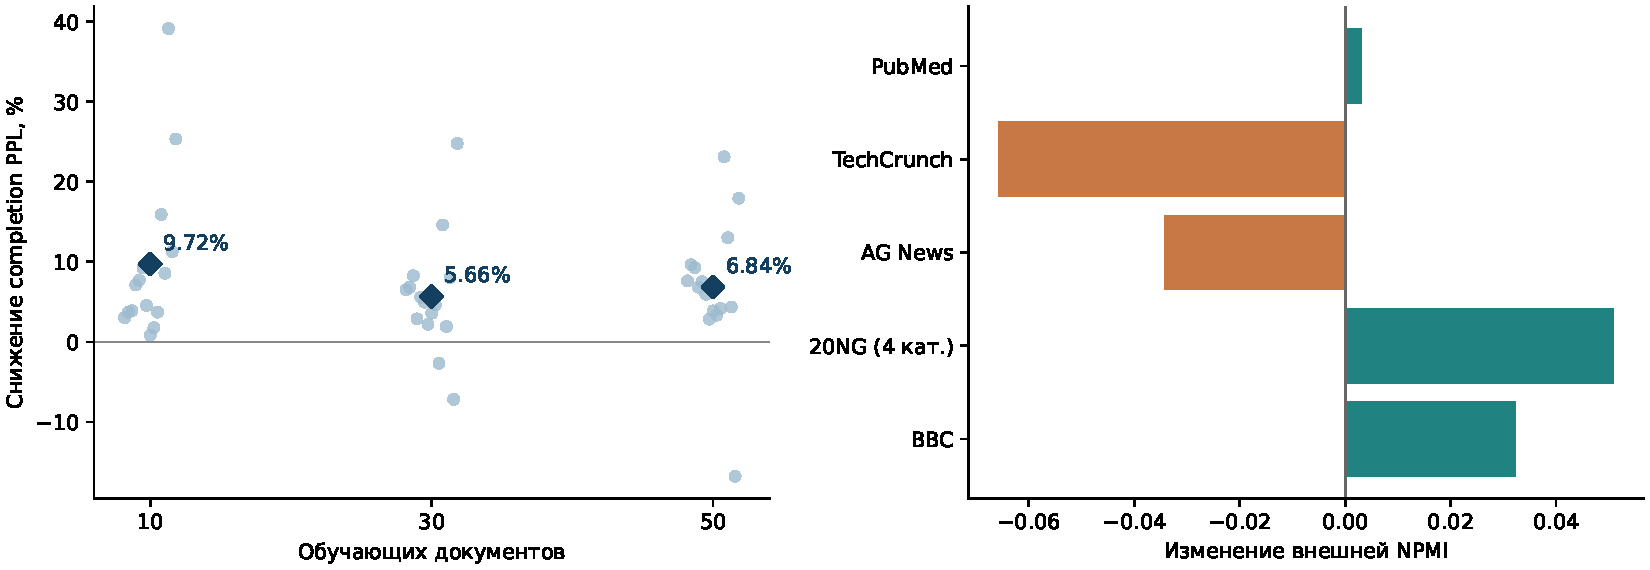
\includegraphics[width=.9\textwidth]{figures/small_effects.pdf}
\caption{Слева --- снижение completion PPL при разных размерах обучения: точки показывают отдельные пары, ромбы --- средние. Справа --- среднее изменение внешней NPMI по корпусам.}
\label{fig:small}
\end{figure}

Абляции на BBC, TechCrunch и PubMed охватывают 27 пар. Полный метод снижает completion PPL на 5.34\%, одна инициализация --- на 5.27\%, только KL --- на 1.14\%, переставленный учитель --- на 0.90\%. Основную часть выигрыша даёт инициализация; дополнительный эффект KL невелик.

На \href{https://www.kaggle.com/datasets/Cornell-University/arxiv}{arXiv} используются 99\,049 документов после фильтрации и общий словарь из 12\,662 слов. Рассматриваются 50, 100, 200, 300 и 500 тем, по четыре seed и 30 итераций AARTM. Обучающая PMI AARTM+Q выше базовой AARTM во всех 20 парах. При 500 темах отношение средних PMI равно 2.03, снижение обучающей PPL --- 2.42\%.
\begin{table}[H]
\centering
\small
\caption{Обучающая PMI на arXiv: среднее $\pm$ выборочное стандартное отклонение по четырём seed.}
\label{tab:arxiv}
\begin{tabular}{lrrrr}
\toprule
$T$ & AARTM & AARTM+Q & FASTopic & CombinedTM+MiniLM \\
\midrule
50 & $0.564\pm0.009$ & $0.679\pm0.010$ & $0.009\pm0.277$ & $-3.887\pm0.701$ \\
100 & $0.599\pm0.025$ & $0.751\pm0.012$ & $-4.948\pm0.791$ & $-5.451\pm0.539$ \\
200 & $0.550\pm0.072$ & $0.761\pm0.016$ & $-6.653\pm0.673$ & $-6.298\pm0.330$ \\
300 & $0.443\pm0.049$ & $0.710\pm0.025$ & $-7.392\pm0.458$ & $-4.077\pm0.560$ \\
500 & $0.271\pm0.028$ & $0.550\pm0.057$ & $-8.062\pm0.442$ & $-1.019\pm0.057$ \\
\bottomrule
\end{tabular}
\end{table}


FASTopic~\cite{wu2024} обучен 30 эпох, CombinedTM~\cite{bianchi2021} --- 100 эпох с MiniLM и общим словарём. При этих настройках AARTM+Q имеет наибольшую обучающую PMI. Однако увеличение обучения FASTopic до 200 эпох в одном запуске повысило его PMI с $-5.759$ до $-0.198$; сходимость CombinedTM отдельно не проверялась. Результат относится к указанным настройкам и обучающим метрикам; тестовой оценки на arXiv нет.

Время AARTM+Q включает построение $Q$ из готовых векторов и обучение, время альтернатив --- обучение. Первичное кодирование не учитывается, поэтому ускорение полного процесса не установлено. CSV, настройки и код пересчёта опубликованы в \url{https://github.com/Estanislavo/llm_tm_kl}.

\FloatBarrier
\begingroup
\small
\bibliographystyle{unsrt}
\bibliography{references}
\endgroup
\end{document}
